\documentclass[11pt]{article}
\usepackage{amsmath, amsthm, amssymb}
\usepackage{array,mathtools}
\usepackage[textwidth=8in,textheight=9in]{geometry}
% \newcommand\showdiv[1]{\overline{\smash{\hstretch{.5}{)}\mkern-3.2mu\hstretch{.5}{)}}#1}}
% \newcommand\ph[1]{\textcolor{white}{#1}}
% \newcommand*{\carry}[1][1]{\overset{#1}}
% \newcolumntype{B}[1]{r*{#1}{@{\,}r}}
\usepackage{listings}
\usepackage{courier}
\setlength{\oddsidemargin}{-1cm}
\setlength{\evensidemargin}{0cm}
\setlength{\textwidth}{500pt}

\usepackage{color}
\usepackage{wrapfig}

\usepackage{listings}
\usepackage{color}

\definecolor{mygreen}{rgb}{0,0.6,0}
\definecolor{mygray}{rgb}{0.5,0.5,0.5}
\definecolor{mymauve}{rgb}{0.58,0,0.82}

\usepackage{courier}

\lstset{basicstyle=\footnotesize\ttfamily,breaklines=true}
\lstset{framextopmargin=50pt,frame=bottomline}


\title{Mega Lit Review}
\author{Luka Milic: lm1015}

\begin{document}
\maketitle
\section{Introduction}
% Most data is unlabeled [http://arxiv.org/abs/1603.08262]
The aim of the project is to implement a neural network which can take both labelled and unlablled face images. \cite{tensorflow2015-whitepaper}
This is relevant to the field of pattern recogintion because real life data is often unlabeled. Infact most learning is unsupervised.
\section{Papers}
\subsection{Shashank}
non-additive effects of multiple AU's, non linear interaction :p
\section{Theory}
Neural networks and stuff\cite{jaiswal_deep_2016}
\section{Model}
\begin{figure}
  \begin{center}
    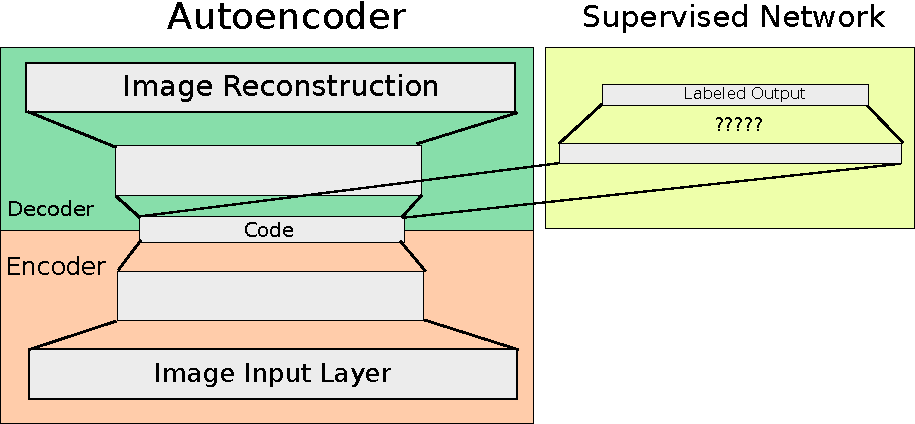
\includegraphics[width=0.5\textwidth]{illustrations/network_01.pdf}
  \end{center}
  \caption{Basic structure of the network}
\end{figure}
really nice models
The idea is to manually set the gradient to zero on unlabled modes. To create a unified cost function so the network can be trained at once.
\section{Data}
DISFA
\section{Evaluation Method}
Need to use some metrics.
\section{Results}
\section{Progress}
\subsection{First target}
implement the basic network with mnist data, compare various cost functions

\bibliographystyle{plain}
\bibliography{bib,bib2}

\end{document}
